\section{Results}
\label{sec:results}
As stated in the introduction, section \ref{sec:intro}, this literature study was complicated by 
the blurring lines between physical, digital, and biological spheres.
This literature study set out to discover the state-of-the-art of research on the energy efficiency impact of, \textbf{explicitly} \textit{robotics software}.
Meaning the explicit impact on energy efficiency of various aspects of the software itself.
It became quickly apparent during the search and selection process, as described in section \ref{sec:study_design:search_selection}, 
that few studies existed on this specific topic.
Out of all 683 potentially relevant studies, only two studies have been found that explicitly research this topic.

\vspace{5mm}

One study \cite{rahman2019cloud_robot_offloading} provides proof that a software architectural change; 
from on-board calculations to off-loading to more available robots or the cloud, actually impacts energy efficiency positively.
Another study \cite{hou2017novel_cloud_evaluation_model} presents a robotics software evaluation method based on energy consumption.
The method allows for identifying those robotics software aspects that consume relatively more energy. 
It can also be used to predict the energy consumption of a specific piece of robotics software, allowing it to be used during software development, 
to create more energy efficient software from the moment it is designed.

\vspace{5mm}

The fact that these two studies were the only ones explicitly covering research into the energy efficiency impact of robotics software aspects will
form the basis of the discussion, given in section \ref{sec:discussion}.
To prevent an insignificant literature study, the focus has been shifted from looking at software aspects, to see what impact 
robotics software in general can have on energy efficiency. The blurred distinction between software and hardware in robotics made the 
application of the inclusion criteria a tough process.
The final selection of primary studies is the result of a rigorous application of these criteria; 
a study had to explicitly cover \textit{some} software aspect in relation to energy efficiency.

\vspace{5mm}

In this section, the insights gained from the data sheet are summarized and given for each column in subsection \ref{sec:results:insights}.
Hereafter, this section is structured according to the research questions.
Each of those subsections gives a detailed explanation of the findings of this literature study in the context of that research question.
The main findings of each research question are presented at the end of each corresponding subsection.

\subsection{Data sheet insights}
\label{sec:results:insights}
The insights, as gained by each of the columns of the data sheet, are given in this subsection.
Any conclusions drawn from these insights in order to answer the research questions targeted by this literature study,
are given in their respective subsections \ref{sec:results:rq1_pub_trends}, \ref{sec:results:rq2_state_of_the_art} and \ref{sec:results:rq3_trade_off}.

\vspace{5mm}

\noindent\textbf{1. Date:}
In figure \ref{fig:pub_trends}, it can be observed that, even though this field of study has been around since before the change of the century,
it truly attained interest in the last decade (2010 - 2020), with a significant spike nearing 2020.
It can also be observed that the more thoroughly peer reviewed, higher quality research; journal articles are only published in the last $\approx$5 years.

\begin{figure}[t]
    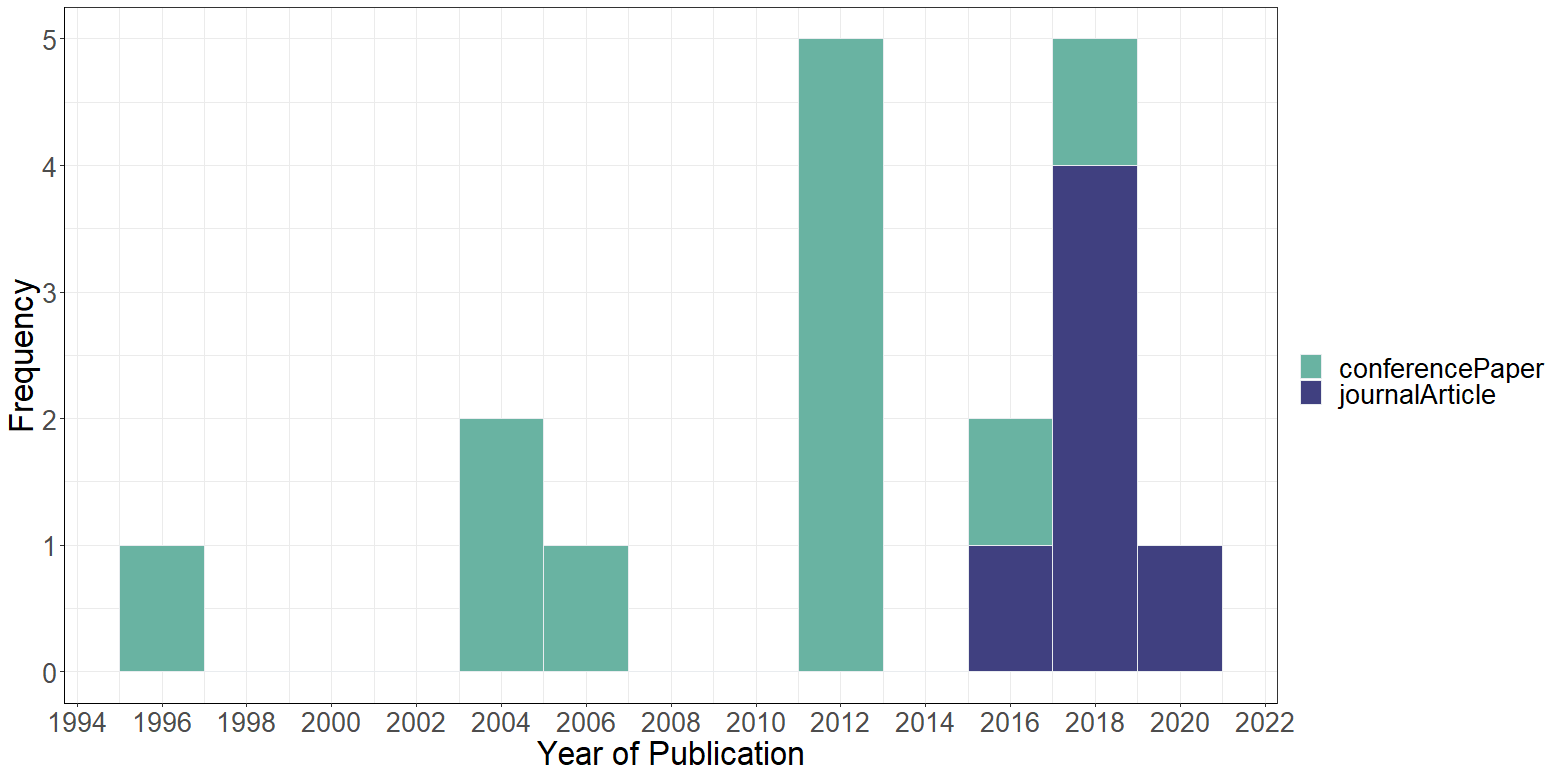
\includegraphics[width=250pt]{figures/publication_trend_extended.png}
    \caption{Publication trends by type}
    \label{fig:pub_trends}
\end{figure}

\vspace{5mm}

\noindent\textbf{2. Energy Metric:}
% Various metrics used
% Power and Energy separate
% Joules / KiloJoules / NanoJoules most popular.
% Most intersting: FPS / W etc.
% Conclusion: Many different metrics, joules most popular, comparison difficult

\vspace{5mm}

\noindent\textbf{3. QA Trade-off:}
% Various trade-offs mentioned.
% Used in RQ 3.

\vspace{5mm}

\noindent\textbf{4. Application Domain:}
% Exploration / Service robots

\vspace{5mm}

\noindent\textbf{5. Identified Major Consumers:}
% Software inefficiencies
% Hardware inefficiencies
% Hardly win-win, only when time reduced, hardware inefficiency reduced etc. (only with software?)

\vspace{5mm}

\noindent\textbf{6. Identified Improving Software Aspect:}
% Mostly solving hardware with software

\vspace{5mm}

\noindent\textbf{7. Major Contribution:}
% For example the entire system, integrating the software aspects to improve inefficiency.

\vspace{5mm}

\noindent\textbf{8. Experiment:}
% Experiment performed most common: simulation, why?

\vspace{5mm}

\noindent\textbf{9. Comparison Against State-Of-The-Art:}
% Mostly yes, important for validity!

\vspace{5mm}

\noindent\textbf{10. Energy Model:}
% Interesting for future research / comparison between the relative studies


\subsection{Results - publication trends (RQ1)}
\label{sec:results:rq1_pub_trends}

In this section the results obtained when analyzing the publication trends on energy efficiency in robotics software are presented.
Understanding the publication trends in the field of study is essential for interpreting the results of this literature study as it gives
an idea of the maturity of the field.

From figure \ref{fig:pub_trends} it can be observed that, even though this field of study has been around since before the change of the century,
it truly attained interest in the last decade (2010 - 2020), with a significant spike nearing 2020.

From these findings we can conclude that the maturity of the field, considering the number of publications relative to their publication dates, 
is rather limited the further back we go in time. It is important to take this into account for both the findings of this literature study, presented in the following subsections 
\ref{sec:results:rq2_state_of_the_art} and \ref{sec:results:rq3_trade_off}, and for the discussion as presented in section \ref{sec:discussion}.
Considering the aforementioned difficulty with the initial goal of this literature study; from the publication trends we can see that this 
is probably the case because of a rather immature field of study.

\vspace{5mm}

\noindent\fcolorbox{black}[HTML]{FFFFFF}{\parbox{0.47\textwidth}{%
\noindent \textbf{Main Findings.}
\begin{enumerate}[nolistsep]
\item The field of study has been around since before the change of the century.
\item However, the field can still be considerd immature as publications only recently attained in numbers.
\item The lack of studies focussing on the energy impact of software aspects of robotics software can be explained by these publication trends.
\end{enumerate}}}

\subsection{Results - state-of-the-art (RQ2)}
\label{sec:results:rq2_state_of_the_art}
In this section the state-of-the-art in analyzing and improving energy efficiency in robotics software is presented as found from studying the primary studies.

\noindent\textbf{1. Analyzing:}
The state-of-the-art in terms of analyzing energy inefficiency would be from study \cite{hou2017novel_cloud_evaluation_model} in which the authors
identify Software as the main component in robotics and thus should also be the main consumer or at least have a significant impact on the
total energy consumption of a robotic system.
For this, the authors developed a method to identify bottlenecks and relatively high consumers in the software of existing systems.
For software that is designed with energy consumption in mind, the authors present a method to be able to predict the energy consumption
of a specific piece of software.

\begin{figure}
    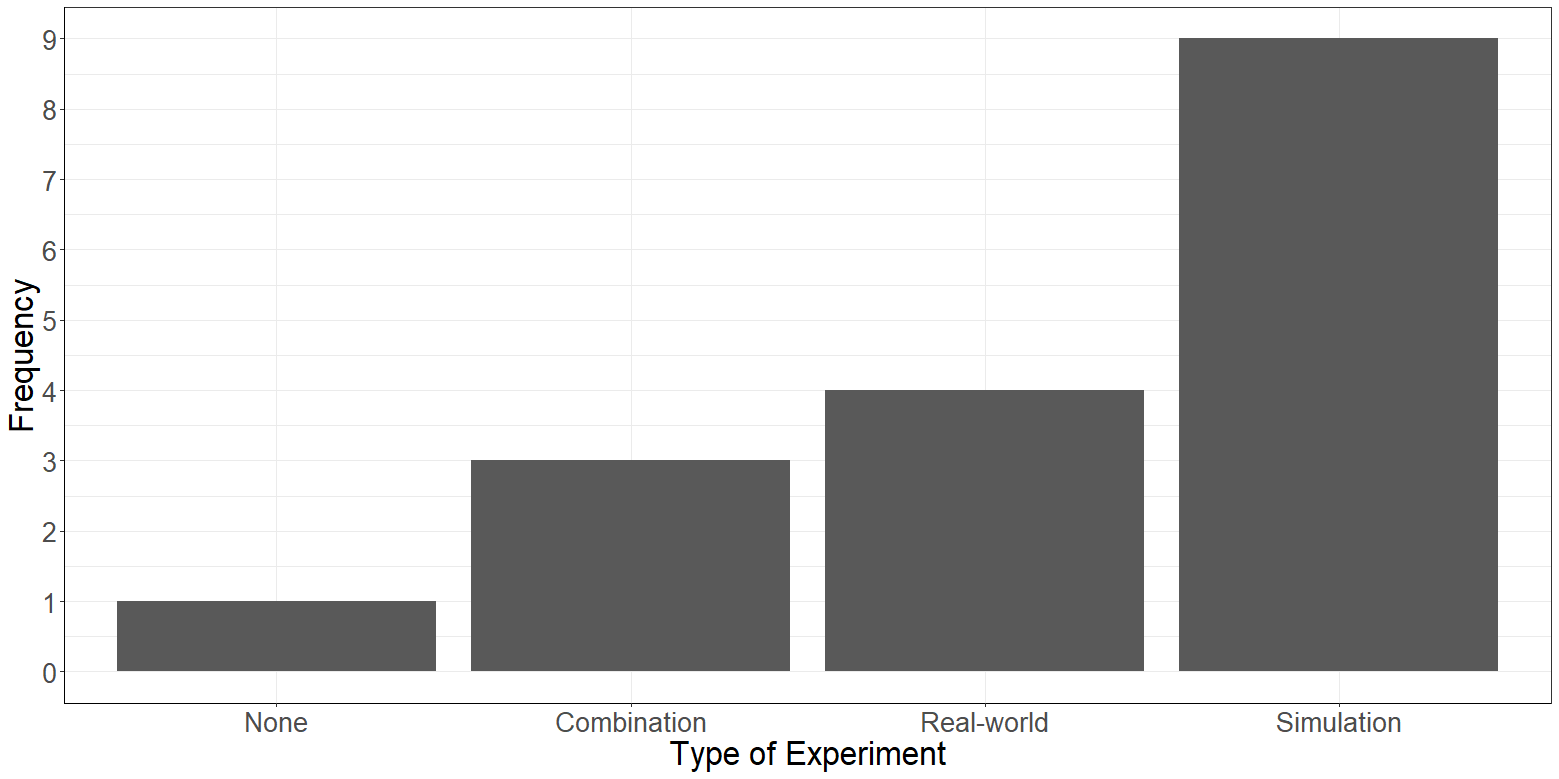
\includegraphics[width=250pt]{figures/experiment_distr.png}
    \caption{Experiment distribution}
    \label{fig:experiment_distr}
\end{figure}

However, it should be considered that this was the only paper that focussed so explicitly on software and its impact on energy.
Considering the 16 other primary studies, we can say that another big standard in this field is the evaluation through practice; 
in the form of a simulation, a real-world experiment or a combination thereof.
From the set of primary studies only study \cite{barili1995efficient_motion} does not feature some form of an experiment.
The relative differences in the measurements taken during an experiment give an idea of the energy efficiency of one method compared to another.
The distribution of experiment types can be observed in figure \ref{fig:experiment_distr}.
It can be observed that a simulation is by far the most popular form of evaluation, used by over $50\%$ of all primary studies.
When considering the combination of simulation and real-world experiments as well, approximately $70\%$ use a simulation as form of evaluation.

An \textbf{energy model} is of course needed when simulating the robotic system. 
For this, many different energy models have been used by the various primary studies, some try to simulate the energy consumption 
as precisely as possible by simulating drag, torque, acceleration, decelleration, etc. with advanced mathematics.

However, many papers have been using a simple energy model.
A concrete example of this can be found in two papers; \cite{patel2012exploration_strategy} and \cite{mei2006mobile_exploration}. 
The first being a study from 2012 and the latter being a study from 2006. 
These papers are written by different authors but within the same field of study; mobile robot exploration.
The model they use consists of a simulated grid, where each grid cell consists of 1x1 Units of Distance, 
and travelling 1 Unit of Distance equals 1 Unit of Energy.
Each stop costs 0.5 Units of Energy and each 45° turn costs 0.4 Units of Energy, each additional 45° adding another 
0.2 Units of Energy to the total cost.
Meaning: a 90° turn would cost 0.6 Units of Energy and a 135° turn would cost 0.8 Units of Energy etc.

If the problem solved is more global (f.e. the path finder is improved) a simple energy model will suffice.
However, when the software presented solves a very local problem, f.e. an improved algorithm for turning a specific type of motor,
a more elaborate, mathematically sound energy model is needed.

\vspace{5mm}

\noindent\textbf{2. Improving:}
The state-of-the-art in improving energy efficiency in robotics software is numerous. 
A trend observed from the primary studies is, however, that they mostly solve hardware (physical) inefficiencies using elaborate
software solutions, like an improved algorithm.
It is however, by definition, not improving energy efficiency in robotics software.
But considering this has been mentioned multiple times, and forms the basis of the discussion in section \ref{sec:discussion}, 
this section will detail what has been found by studying the primary studies in the context of improving energy efficiency 
by \textit{using} robotics software in general.

The state-of-the-art in improving energy efficiency in robotics software is numerous, the prime examples are given here.
Each primary study presented an evaluated software solution that improves energy efficiency in one specific way.
If one would apply all applicable paradigms to a robotic system, 
the energy efficiency of that robotic system is guaranteed to be significantly improved.
The prime examples consist of:

- The notion of off-loading computations to other, nearby, robots that are more 'available' 
(i.e. robots that have more resources available for such computations relative to the current one.), or to off-load it to the cloud.
The concept here is that the cloud infrastructure is more optimized, and will thus result in an improved energy efficiency. 
Also, a nearby robot that is more 'available' has just as much computational power as the current robot, and the same energy efficiency
but as the latency between the current robot and the nearby robot is lower than that with the cloud infrastructure a severe trade-off between
Timeliness and Efficiency can be prevented.
Eventhough some energy is wasted in the transmission of data, the overall energy consumption is decreased \cite{rahman2019cloud_robot_offloading}.
    
- The notion of improving the path finding for mobile robot exploration. 
Many existing studies select the next target based on the utilities and costs of the frontier cells 
\cite{burgard2005multi_robot_exploration, simmons2000multi_robot_exploration,zlot2002multi_robot_exploration} 
However, study \cite{mei2006mobile_exploration} proves that if the next target is selected based on the orientation of the robot, 
that overlap in the robot trajectory is guaranteed to be impossible. This decreases inefficiency by nature, and thus improves energy 
efficiency.

- The notion that limiting stops, turns, directional changes and the degree to which the direction is changed as much as possible 
significantly improves energy efficiency. By the very nature of this notion, an improved obstacle detection and avoidance algorithm
is needed for mobile robotic systems. This notion is widespread over the primary studies, and presented and evaluated in 
\cite{xie2018mecanum_wheel, kim2016firefighting_robot, benkrid2016multi_robot_exploration, barili1995efficient_motion, 
jia2004grid_strategy_exploration, mei2005energy_consumers_identified, patel2012exploration_strategy}.

- The notion that motion at high speeds, with numerous moments of acceleration and decelleration is to be prevented
\cite{wingstrom2013robot_cell_scheduling}.

- The notion that idle time should be prevented as much as possible \cite{gurel2019industrial_robot_scheduling, 
kaitwanidvilai2020industrial_robot_cycle_time, wingstrom2013robot_cell_scheduling}.

- The notion of applying well-accepted Computer Science paradigms, like the popular MapReduce paradigm for distributed systems,
to multi-robot systems. Limiting data traffic using MapReduce \cite{huh2013distributed_swarm}.

- The notion of limiting physical inefficiencies, like the loss of traction, by using an elaborate software solution.
Like adding subrobots communicating using distributed systems paradigms \cite{kim2016firefighting_robot}.

- The notion that the use of more advanced hardware (i.e. more optimised, desktop grade, hardware instead of custom robotic hardware) 
on robots in combination with optimised software improves energy efficiency significantly \cite{cheng2018FPGA_image_recognition}.

- The notion that sacrificing some energy on finding a better position for the transmission of data over a wireless connection
(a higher channel gain) will ultimately improve energy efficiency as less time is spend and wasted on (re)transmitting 
data over a bad wireless connection \cite{licea2013wireless_comms}.

\vspace{5mm}

\noindent\fcolorbox{black}[HTML]{FFFFFF}{\parbox{0.47\textwidth}{%
\noindent \textbf{Main Findings.}
\begin{enumerate}[nolistsep]
\item The state-of-the-art on analyzing the energy efficiency of robotics software is provided by \cite{hou2017novel_cloud_evaluation_model}, allowing for the identification of bottlenecks in software and the prediction of energy consumption of a piece of software.
\item However, the most common way to analyze the energy efficiency of robotics software consists of performing experiments, evaluating the results.
\item The state-of-the-art on improving the energy efficiency is numerous, but generally consists of:
    \begin{enumerate}
        \item Off-loading computations to optimised infrastructure.
        \item The application of well-accepted, well-established Computer Science paradigms, like the popular MapReduce paradigm for distributed systems.
        \item Improved path finding, obstacle avoidance etc.
        \item Limit physical inefficiencies, idle time, acceleration, decelleration, stops, turns, directional changes and the extent of the directional change.
        \item The use of more optimised hardware.
        \item Sacrificing some energy to achieve higher efficiency, f.e. finding a better location with better signal for data transmission.
    \end{enumerate}
\end{enumerate}}}

\subsection{Results - energy QA trade-off (RQ3)}
\label{sec:results:rq3_trade_off}
From the primary studies it became quickly apparent that no significant improvement of energy efficiency came without the cost
to some other attribute. These trade-offs have been mapped to 
\textit{system Quality Attributes\cite{iso2011quality_attributes}} and will be presented
in this section.

This section aims to give insight into the various costs that have been associated with improving energy efficiency.
Any reader can judge if any QA trade-off is manageable in the context of their own system, when applying the paradigms
described in subsection \ref{sec:results:rq2_state_of_the_art}. 
The QA's that trade-off with improving energy efficiency are further detailed and related to findings from the primary studies below.

\begin{figure}
    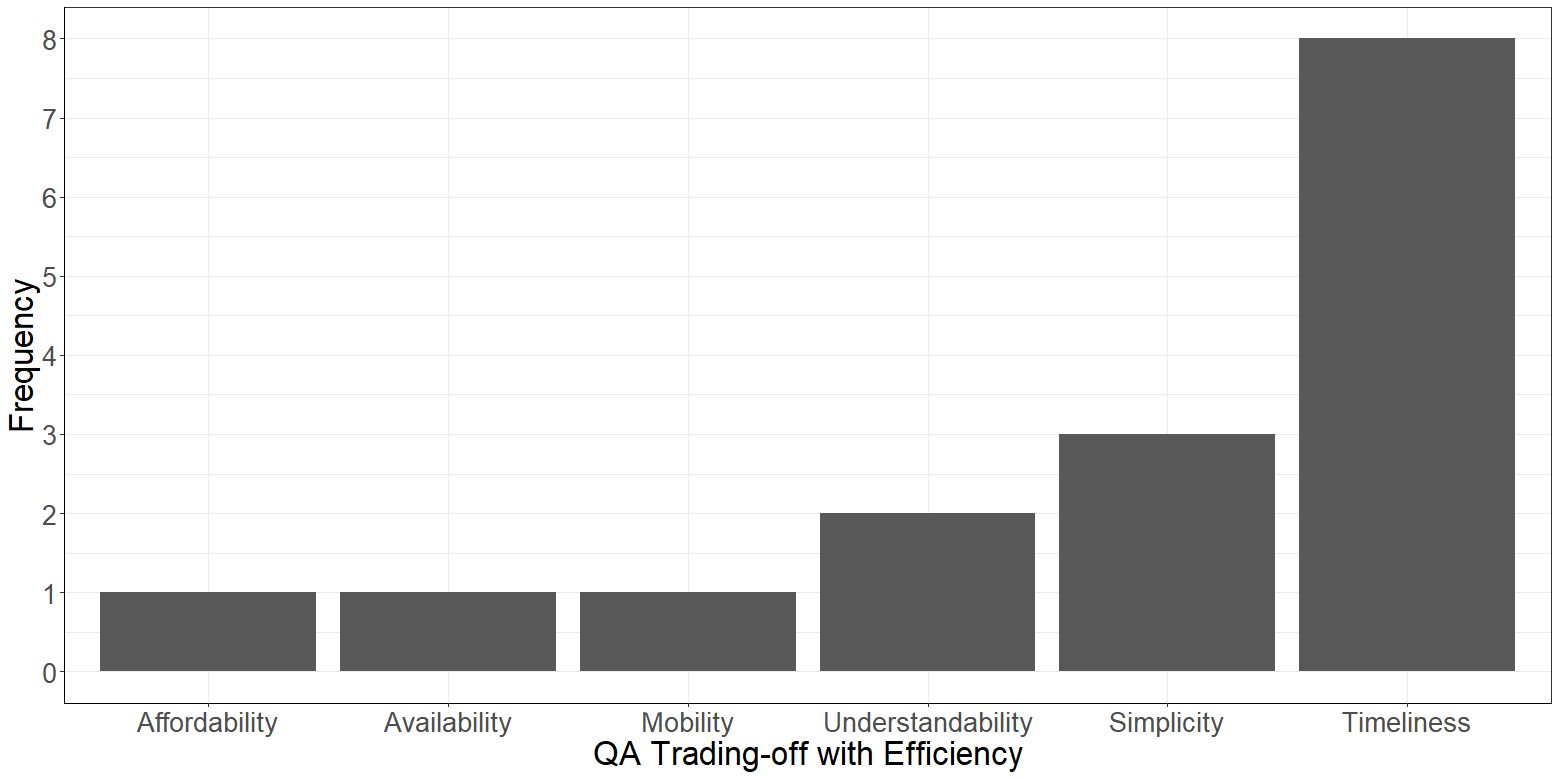
\includegraphics[width=250pt]{figures/trade_off_freq.png}
    \caption{QA Trade-off with Efficiency frequency distribution}
    \label{fig:trade_off_freq}
\end{figure}

\vspace{5mm}

It can be observed from figure \ref{fig:trade_off_freq} that the most common QA to trade-off with Efficiency is \textbf{Timeliness}.
This is to be expected as one can reason with common sense that when, f.e. speed is decreased to increase Efficiency, Timeliness will decrease.

Under Timeliness one could also understand the notion of \textit{Performance}, but considering that this is not an official
system's Quality Attribute, it can be explained as Timeliness.

- \textbf{Affordability} trades-off with Efficiency as improving Efficiency can require an increase in cost for the developer.
For example, the addition of subrobots to reduce the loss of traction by the weight of the payload.

- \textbf{Availability} trades-off with Efficiency as improving Efficiency can require the robot to reject stimuli when it predicts
that the stimuli will cost too much or waste energy \cite{kirtay2013humanoid_emotion}.

- \textbf{Mobility} trades-off with Efficiency as improving Efficiency can require the robot to limit stops, turns, directional changes and the degree 
to which the direction is changed as much as possible. This significantly reduces the Mobility of the robot.

- \textbf{Understandability} trades-off with Efficiency as improving Efficiency can require the robot to be more complicated in terms of hardware
and/or software. 
The added complexity; like an improved, more complex, algorithm which improves energy efficiency, can reduce the Understandability of the system.

- \textbf{Simplicity} trades-off with Efficiency as improving Efficiency can require the system to be expanded in a trivial manner, thus not
reducing the Understandability of the system but nonetheless making it more complex. Like adding the aforementioned subrobots to the system.

- \textbf{Timeliness} trades-off with Efficiency as improving Efficiency can require the robot to take the longer route instead of the shortest route
as the shortest route might contain more stops and turns, which is to be limited as much as possible.

\vspace{5mm}

Besides the fact that certain QA's need to be traded-off in order to improve energy efficiency, the extent to which this is required 
matters just as much, if not more.
For each system, the hit to the traded-off QA and the improvement of Efficiency will be significantly different.
Thus, an indication of expected percentages cannot be given.
However, with common sense it can be reasoned that a disproportional hit to the traded-off QA relative to the increase in Efficiency might not be worthwile.

Study \cite{kaitwanidvilai2020industrial_robot_cycle_time} for example states: "This method reduces energy consumption from 8155.20 to 7148.6 J, 
a decrease of 12.3\%.  On the other hand, the total moving time is increased by 71.8\% from 6.60 to 11.34 s". 
In case the system in question can suffer a 71.8\% reduction in Timeliness for a 12.3\% increase in Efficiency, it might be worthwile.
However, it can be considered a good example of a trade-off which might not be worthwile for most systems, let alone time-critical systems.

\vspace{5mm}

\noindent\fcolorbox{black}[HTML]{FFFFFF}{\parbox{0.47\textwidth}{%
\noindent \textbf{Main Findings.}
\begin{enumerate}[nolistsep]
\item The most common QA trade-off relative to Efficiency is \textbf{Timeliness}.
\item Some studies present QA trade-offs which are easily worthwile, like the reduction of Simplicity in favor of an increase in Efficiency.
\item Some QA trade-offs are not worthwhile for most robotic systems, like the reported 12.3\% increase in Efficiency for a 71.8\% decrease in Timeliness.
\end{enumerate}}}
